\documentclass[12pt,a4paper]{article}
\usepackage{graphicx}
\usepackage{amsmath}
\usepackage{amssymb}
\usepackage[hidelinks]{hyperref}
\usepackage[margin=1.3in]{geometry}
\usepackage{placeins}
\usepackage{float}
\usepackage[style=authoryear,backend=biber,maxbibnames=6]{biblatex}
\usepackage{booktabs}
\usepackage{array}
\usepackage{caption}
\usepackage{subcaption}
\usepackage{setspace}
\usepackage{parskip}
\usepackage{microtype}
\usepackage{algorithm}
\usepackage{algpseudocode}
\usepackage{xcolor}

\emergencystretch=1em

\addbibresource{ref.bib}

\onehalfspacing

\title{\textbf{Cost-Sensitive Electricity Demand Forecasting\\
via Asymmetric Loss Optimisation}\\[0.6em]
\large Beyond the Linear Newsvendor Framework}
\author{[Author Names]}
\date{March 2026}

\begin{document}

\maketitle

\begin{abstract}
Accurate electricity demand forecasting is critical for market participants in
deregulated power markets, where procurement decisions must be made before
actual demand is observed.  
Traditional forecasting approaches minimise symmetric
loss functions such as mean squared error (MSE), which implicitly treat over- and
under-prediction as equally costly.  In practice the costs of under-predicting
demand --- triggering emergency reserve activation, load shedding, or costly
real-time purchases --- substantially exceed those of over-prediction.  
We formalise this asymmetry through an explicit cost function and incorporate it
directly into the training objective, replacing symmetric loss functions with a
cost-sensitive alternative.  Concretely, we train a feedforward neural network with an asymmetric loss function that directly targets
the cost-minimising prediction under the prevailing cost structure.  Using a dataset of daily electricity demand in
Israel spanning March~2023 to February~2026, augmented with meteorological data
from three major cities, we evaluate our approach against MSE-trained baseline models.  Synthetic asymmetric cost functions are
generated to assess performance across a range of cost scenarios.  Our results
demonstrate that cost-aware training leads to statistically significant
reductions in operational cost compared to symmetric baselines, and that MSE is a
poor surrogate for operational cost under asymmetric loss.
We benchmark against the \emph{real} day-ahead forecasts published by the Israeli
system operator Noga: although predictive accuracy was not our objective, our
practical, open-source model improves on this operational forecast even under
symmetric error metrics, while additionally delivering an economic benefit we
argue is realistic to adopt.
\end{abstract}

\setcounter{tocdepth}{2}
\tableofcontents
\newpage

\section{Introduction}\label{sec:intro}
The modern electricity grid operates through wholesale markets in which
producers and large consumers interact---directly or through a central
operator---to determine how much power is generated and consumed.  In a
stylised day-ahead market, producers submit offers specifying the quantities of
electricity they are willing to supply at various price points, while suppliers
(and possibly a handful of very large consumers) submit corresponding demand
bids.  A system operator then clears the system by finding the price at which
aggregate supply equals aggregate demand, setting a single clearing price for
each settlement period (typically one hour).  This mechanism promotes economic
efficiency by rewarding low-cost producers and incentivising demand
response~\parencite{stoft2002power, kirschen2018fundamentals}.

Real markets differ considerably in how centralised this process is.  The
Israeli market, which is the setting of this study, is comparatively
centralised: the system operator (Noga) forecasts national demand for each hour
of the following day, and this day-ahead forecast---together with the resulting
price signal---determines how much electricity producers are scheduled to
deliver in each settlement period.  The process is therefore less the
continuously cleared double auction of textbook descriptions and more a
coordinated, forecast-driven dispatch.  Regardless of the precise market design,
however, the day-ahead demand forecast is the pivotal quantity: it is fixed
before real-time demand is known, and its accuracy propagates directly into
generation scheduling and price.

A central challenge in this architecture is that procurement decisions must be
finalised a day in advance, before actual real-time demand is known.  The
accuracy of demand forecasts therefore directly affects the operational
decisions and financial outcomes of all market participants.  It remains an open
question to what extent individual suppliers maintain their own demand models.  A
plausible account of current practice is that, once the operator publishes its
day-ahead demand forecast, each supplier simply draws its own share from that
forecast based on experience, and the market settles on a relatively stable price
that is reasonable on average but may embed sizeable, systematic error margins.
If so, more sophisticated forecasting---whether by the suppliers or by the system
operator---could translate into lower retail prices, which is part of what
motivates the present work.

A system operator that accurately anticipates demand can procure the right
amount of energy at competitive prices.  Inaccurate forecasts, by contrast,
force participants into costly corrective actions in the balancing or real-time
markets, where prices can be dramatically different from day-ahead levels.  It is
worth stressing that these price differences arise from two distinct sources of
uncertainty: errors in predicting \emph{demand}, and errors in predicting
available \emph{production capacity}---the latter being especially pronounced in
systems that rely heavily on variable renewable generation such as solar and
wind~\parencite{morales2014integrating}.  This paper is concerned exclusively
with the first source, uncertainty in day-ahead demand; production-side
uncertainty, while important, is outside our scope.

\subsection{Asymmetric Costs in Electricity Markets}

A critical and often overlooked aspect of electricity demand forecasting is the
\emph{asymmetry} of the costs associated with forecast errors.  When demand is
\emph{overestimated}, the system operator or retailer procures more electricity
than is ultimately needed.  The excess supply can typically be sold back into the
balancing market, curtailed, or stored (if storage is available), resulting in a
relatively modest financial loss.  In deregulated markets with well-functioning
balancing mechanisms, the per-unit cost of over-procurement is generally bounded
and predictable.

When demand is \emph{underestimated}, the cost of error is usually much higher.
The system operator must source additional electricity in the real-time market at
short notice to prevent blackouts.  Real-time prices are typically highly
volatile and can spike to several multiples of the day-ahead price during periods
of scarcity.  In extreme cases, the system may lack sufficient reserve capacity
to meet demand, triggering involuntary load shedding, emergency imports, or the
activation of expensive peaking units.  Beyond the direct financial costs, supply
shortfalls carry significant reliability and regulatory
implications~\parencite{stoft2002power, kirschen2018fundamentals}.

Empirical studies in various electricity markets suggest that the ratio of
under-procurement costs to over-procurement costs, $c_u / c_o$, typically lies in
the range $[5,\,20]$, depending on market structure, regulatory context, and the
availability of real-time resources~\parencite{zhang2022costoriented}.  This
asymmetry fundamentally changes the optimal forecasting problem: rather than
seeking a prediction that minimises expected squared error, a rational market
participant should seek a prediction that minimises expected asymmetric cost.

This decision-theoretic view has developed alongside a substantial body of work
on electricity forecasting more broadly.  \textcite{weron2014electricity}
provides a comprehensive review of the state of the art in electricity price
forecasting, surveying statistical, machine-learning, and hybrid approaches.
While its focus is on price rather than demand, the review highlights the central
role of model selection, loss-function choice, and benchmark comparisons that
also apply in the load-forecasting context.

\textcite{hong2016probabilistic} offer a tutorial review of probabilistic
electric load forecasting, covering methods ranging from regression-based
quantile estimation to ensemble and Bayesian approaches.  Crucially, they argue
that point forecasts are insufficient for operational decision-making and
advocate for full predictive distributions or at least prediction intervals---a
view consistent with the quantile-forecasting objective we adopt.

The practical importance of probabilistic evaluation metrics, and of the pinball
loss in particular, was cemented by the Global Energy Forecasting Competition
2014~\parencite{hong2016gefcom2014}.  GEFCom2014 was the first major forecasting
competition to use pinball loss as its primary scoring rule across the
electricity load, price, wind, and solar tracks.  It established pinball loss as a
community standard and demonstrated that models explicitly optimised for quantile
accuracy substantially outperform those adjusted only post-hoc.

Despite the theoretical clarity of this framing, the majority of practical
forecasting systems in electricity markets continue to use symmetric loss
functions---most commonly MSE or mean absolute error (MAE)---both for training
predictive models and for evaluating their performance.  This disconnect between
training objective and operational cost constitutes a systematic source of
suboptimality that has received growing attention in the academic
literature~\parencite{wang2019pinball, lin2020asymmetric, wu2021svr,
zhang2022costoriented} but has yet to see widespread adoption in practice.

\subsection{Cost-Oriented and Asymmetric Learning for Load Forecasting}

The theoretical foundation for prediction under asymmetric costs was laid by
\textcite{koenker1978regression}, who introduced \emph{regression quantiles} as a
natural generalisation of sample quantiles to the linear model.  They showed that
minimising the asymmetric pinball loss (equivalently, the ``check function'')
yields an estimator of the conditional $\tau$-quantile of the response, and
established its asymptotic properties.  This result directly underpins our use of
a cost-sensitive asymmetric loss function---instantiated as a non-linear variant
of the pinball loss---as the training objective for day-ahead demand forecasting.

\textcite{christoffersen1997optimal} provided the corresponding
decision-theoretic foundation.  They showed that under a general asymmetric loss
function the optimal point forecast is \emph{biased}, and that the optimal amount
of bias is time-varying and depends on higher-order conditional moments such as
conditional variance.  In particular, their analysis implies that any forecast
trained with a symmetric objective (e.g.\ MSE) will be systematically suboptimal
when the true cost structure is asymmetric, even if the conditional mean is
estimated perfectly.

Building on these foundations, a more recent line of work addresses the mismatch
between symmetric training objectives and asymmetric operational costs directly
in the electricity setting, embedding the cost asymmetry into the learning
objective itself rather than correcting for it after the fact.

\textcite{wang2019pinball} train a Long Short-Term Memory (LSTM) network directly
with the pinball loss to produce probabilistic individual load forecasts.  By
guiding the network to minimise $\mathbb{E}[\mathcal{L}_\tau]$ rather than MSE,
their approach yields calibrated quantile predictions without requiring post-hoc
quantile regression on the residuals.  Their results show improved reliability and
sharpness compared to symmetric-loss baselines.

\textcite{lin2020asymmetric} address the related problem of contract-capacity
optimisation for high-voltage consumers, where the electricity pricing structure
is inherently asymmetric: underestimating demand triggers penalty charges at a
higher per-unit rate than overestimating.  They propose several asymmetric loss
functions derived directly from the Taiwan Power Company's pricing formula, and
demonstrate that LSTM models trained with these loss functions reduce electricity
costs by 0.88\%--2.42\% over symmetric MSE baselines.

\textcite{wu2021svr} extend this idea to support vector regression (SVR),
developing a cost-oriented asymmetric SVR (AsySVR) framework based on a
linear-linear loss function with an insensitivity parameter to improve
generalisation.  Evaluated on New South Wales load data, their asymmetric
framework achieves daily economic cost reductions of 42\%--57\% relative to
standard SVR, underscoring that the choice of loss function can have a large
practical impact on operational outcomes.

\textcite{zhang2022costoriented} further formalise the decision-oriented
perspective on load forecasting, framing the problem explicitly in terms of the
downstream cost incurred by the system operator.  Their cost-oriented framework
bridges the gap between forecast-accuracy metrics and operational objectives, and
provides theoretical justification for replacing standard point-forecast losses
with cost-aware alternatives.

Taken together, this body of work establishes that asymmetric, cost-sensitive
training objectives are both theoretically motivated and empirically superior to
symmetric alternatives in electricity applications.  Two gaps, however, remain.
First, existing studies almost exclusively employ \emph{piecewise-linear}
asymmetric losses---the pinball loss, or the linear-linear penalties derived from
a specific tariff---and thus inherit the newsvendor model's linearity assumption,
even though real procurement costs are frequently non-linear.  Second, and more
practically, these methods are typically benchmarked against statistical
baselines rather than against the forecast an experienced system operator
actually deploys, leaving open whether cost-aware training improves upon a strong,
real-world operational forecast.

Our work is designed to close both gaps.  We formulate the forecasting problem
with a general, not-necessarily-linear asymmetric cost function that subsumes the
pinball loss as a special case, and train a neural network to minimise it
end-to-end.  Crucially, we evaluate against the \emph{real} day-ahead forecasts
published by the Israeli system operator Noga---an operational baseline with
access to proprietary data and domain expertise---rather than against a synthetic
statistical model.  This lets us ask not merely whether cost-aware training beats
a symmetric loss in the abstract, but whether it can improve upon the forecast
currently used to help run a national grid.  The cost-minimising quantile that
this training targets is characterised formally in Section~\ref{sec:modeling}.

\subsection{Contributions}

The contributions of this paper are as follows:

\begin{enumerate}
    \item \textbf{A general asymmetric-cost formulation.}  We formulate day-ahead
          demand forecasting under a general, not-necessarily-linear asymmetric
          cost function that subsumes the pinball loss as a special case, and we
          train a feedforward neural network to minimise it end-to-end
          (Sections~\ref{sec:modeling}--\ref{sec:method}).

    \item \textbf{Evaluation against a real operational forecast.}  Rather than
          benchmarking against a synthetic statistical baseline, we compare
          against the \emph{actual} day-ahead forecasts published by the Israeli
          system operator Noga --- a strong, real-world baseline produced with
          proprietary data and domain expertise.

    \item \textbf{A practical model that improves on the operator's forecast.}
          Although raw predictive accuracy was \emph{not} a goal of this work,
          our model outperforms the Noga forecast not only on cost-sensitive
          metrics but even under symmetric error metrics such as mean squared
          error.  We regard this as an incidental by-product of a deliberately
          simple architecture and believe that substantial further improvement
          is readily achievable.

    \item \textbf{A demonstration of economic impact.}  We quantify the
          operational cost reduction that cost-aware training delivers over
          symmetric baselines across a range of cost scenarios, showing an effect
          that is large enough --- and cheap enough to obtain --- to be practical
          to adopt in a live market setting.

    \item \textbf{An open-source implementation.}  We release our complete code
          and data pipeline, from raw data ingestion through model training and
          evaluation, as open source,\footnote{\url{https://github.com/gkutiel/noga}}
          so that our results can be reproduced and extended.
\end{enumerate}


\section{Cost-Sensitive Forecasting: Problem Formulation and Asymmetric Loss}%
\label{sec:modeling}
\subsection{Problem Formulation}

In day-ahead electricity demand forecasting, the system operator must commit to a
procurement quantity $p$ before observing actual demand $X$.  We model $X$ as a
random variable whose distribution is \emph{unknown} and must be inferred from
data; we make no parametric assumption about its form.

\paragraph{Assumptions.}  We adopt the following assumptions, which are mild and
operationally grounded:

\begin{enumerate}
    \item \textbf{Asymmetry.}  Under-prediction is more costly than
          over-prediction of equal magnitude: the costs incurred when actual
          demand exceeds the forecast are larger than those incurred when the
          forecast exceeds actual demand ($c_u > c_o > 0$).

    \item \textbf{Monotonicity.}  Costs are non-decreasing in the magnitude of
          the prediction error: larger errors are never cheaper than smaller
          errors, in either direction.

    \item \textbf{Known, differentiable costs.}  For the purposes of this paper
          we assume that the cost functions are known and differentiable, so they
          can be incorporated directly as training objectives for gradient-based
          optimisers.
\end{enumerate}

\paragraph{Cost structure.}  Let $\ell_o:\mathbb{R}_{\geq 0}\to\mathbb{R}_{\geq
0}$ and $\ell_u:\mathbb{R}_{\geq 0}\to\mathbb{R}_{\geq 0}$ denote the cost
functions for over- and under-prediction respectively, where the argument is the
magnitude of the error.  
The total realised cost of procurement decision $p$ against actual demand $X$ is:

\begin{equation}
    C(p, X) =
    \begin{cases}
        \ell_o(p - X) & \text{if } X \leq p \quad \text{(over-prediction)} \\
        \ell_u(X - p) & \text{if } X > p \quad \text{(under-prediction)}
    \end{cases}
    \label{eq:cost}
\end{equation}

\paragraph{Goal.}  The objective is to find a procurement decision $p^*$ that
minimises the \emph{expected cost}, and not the expected prediction error.

\paragraph{The Newsvendor Special Case:}
\label{sec:newsvendor}

to gain analytical insight, we first consider the classical special case in which
costs are \emph{linear} 
the setting of the \emph{newsvendor model}~\cite{arrow1951optimal}, a classical
inventory-theoretic framework in which a decision-maker commits to a quantity
before demand is realised.  
Let $c_o>0$ and $c_u > c_o$ be the per-unit overage
and underage costs.

This is a well known problem in which the optimal procurement level is given by the critical fractile formula:
\begin{equation}
    p^* = F^{-1}\!\left(\frac{c_u}{c_u + c_o}\right)
    \label{eq:optimal_threshold}
\end{equation}

\subsection{Limitations of the Linear Newsvendor Framework}%
\label{sec:limitations_nv}

While the newsvendor model provides a tractable and theoretically grounded
formulation, it does not always capture the complexities of real-world electricity markets.  

Our general formulation (Equation~\eqref{eq:cost}) addresses this limitation:
it does not assume linear costs and it does not require knowledge of the demand
distribution, relying instead on empirical samples via the training loss.

\subsection{Synthetic Cost Functions for Evaluation}

Since we do not have access to actual cost data from the electricity market
operator, we evaluate our models against \emph{synthetic} cost functions that
satisfy the qualitative properties stated in the problem formulation.

For simplicity, we conduct our main evaluation using two \emph{pinball loss}
functions with under/over-prediction cost ratios of $1\!:\!5$ and $1\!:\!20$
respectively.  These ratios are consistent with the findings of prior work on
asymmetric costs in electricity demand forecasting, which reports that the cost
of under-prediction typically exceeds the cost of over-prediction by a factor of
five to twenty~\cite{weron2014electricity}.  Pinball losses are piecewise linear
and widely used in quantile regression, making them a natural and interpretable
baseline for cost-sensitive evaluation.




\section{Methods}\label{sec:method}
The objective of this study is to determine whether a demand forecaster trained
end-to-end to minimise an \emph{asymmetric operational cost} can outperform both
a symmetric-loss model and the real operational forecast of the Israeli system
operator, under the cost asymmetries characteristic of electricity procurement.
This section describes the material and procedures used to answer that question:
the dataset (Section~\ref{sec:dataset}), the neural architecture and the three
training objectives we compare, and the protocol under which they are evaluated
(Section~\ref{sec:model-training}).

\subsection{Dataset}
\label{sec:dataset}
In this section we describe the dataset we used for our experiments. 
The dataset consists of both electricity consumption and weather data, collected from various sources. 
The electricity consumption data was obtained from the Israeli electricity system operator Noga~(\cite{noga}), 
while the weather data was sourced from a nearby meteorological station~(\cite{ims}).
Electricity consumption data includes hourly readings of power usage.
Crucially, it also includes the \emph{real day-ahead forecasts} published by Noga as part of the
market clearing process.  These are the actual forecasts used by the system operator in the
day-ahead market, not post-hoc reconstructions.  Their inclusion in our dataset
provides two important opportunities: (i)~we can directly compare the performance
of our learned models against the operational forecasts actually used in the market,
serving as a strong real-world baseline; and (ii)~we can analyze the
distribution of real-world prediction errors produced by an experienced operator,
which motivates and contextualizes the cost asymmetries studied in this paper.
The weather data includes temperature, humidity, and wind speed measurements taken every three hours in the three major cities of Israel: Tel Aviv, Jerusalem, and Haifa.
% Table~\ref{tab:electricity-fields} summarizes the fields present in the electricity consumption data,
% and Table~\ref{tab:weather-fields} summarizes the fields present in the weather data. 
% The dataset covers the period from March 2023 to February 2026, 
% providing a comprehensive view of electricity consumption patterns 
% and their relationship with weather conditions over the course of almost three years.

% \begin{table}[ht]
%     \centering
%     \begin{tabular}{ll}
%         \hline
%         \textbf{Field} & \textbf{Description} \\
%         \hline
%         \texttt{date} & Calendar date (DD-MM-YYYY). \\
%         \texttt{total\_demand} & Total daily electricity demand (MWh). \\
%         \texttt{total\_day\_ahead\_forecast} & Operator's day-ahead forecast (MWh). \\
%         \hline
%     \end{tabular}
%     \caption{Electricity consumption data fields (daily aggregated from hourly source data).}
%     \label{tab:electricity-fields}
% \end{table}

% \begin{table}[ht]
%     \centering
%     \begin{tabular}{ll}
%         \hline
%         \textbf{Field} & \textbf{Description} \\
%         \hline
%         \texttt{temperature\_Haifa} & Daily mean temperature, Haifa ($^\circ$C). \\
%         \texttt{temperature\_Jerusalem} & Daily mean temperature, Jerusalem ($^\circ$C). \\
%         \texttt{temperature\_Tel\_Aviv} & Daily mean temperature, Tel~Aviv ($^\circ$C). \\
%         \hline
%     \end{tabular}
%     \caption{Weather data fields (daily means aggregated from tri-hourly station observations).}
%     \label{tab:weather-fields}
% \end{table}

\subsection{Data Analysis}
To better understand the dataset, we performed an exploratory data analysis (EDA) to identify patterns and relationships between the electricity consumption and weather data.
Figure~\ref{fig:daily-demand} shows the daily electricity consumption over the course of the dataset alongside the daily average temperature in Tel Aviv.

\begin{figure}[ht]
    \centering
    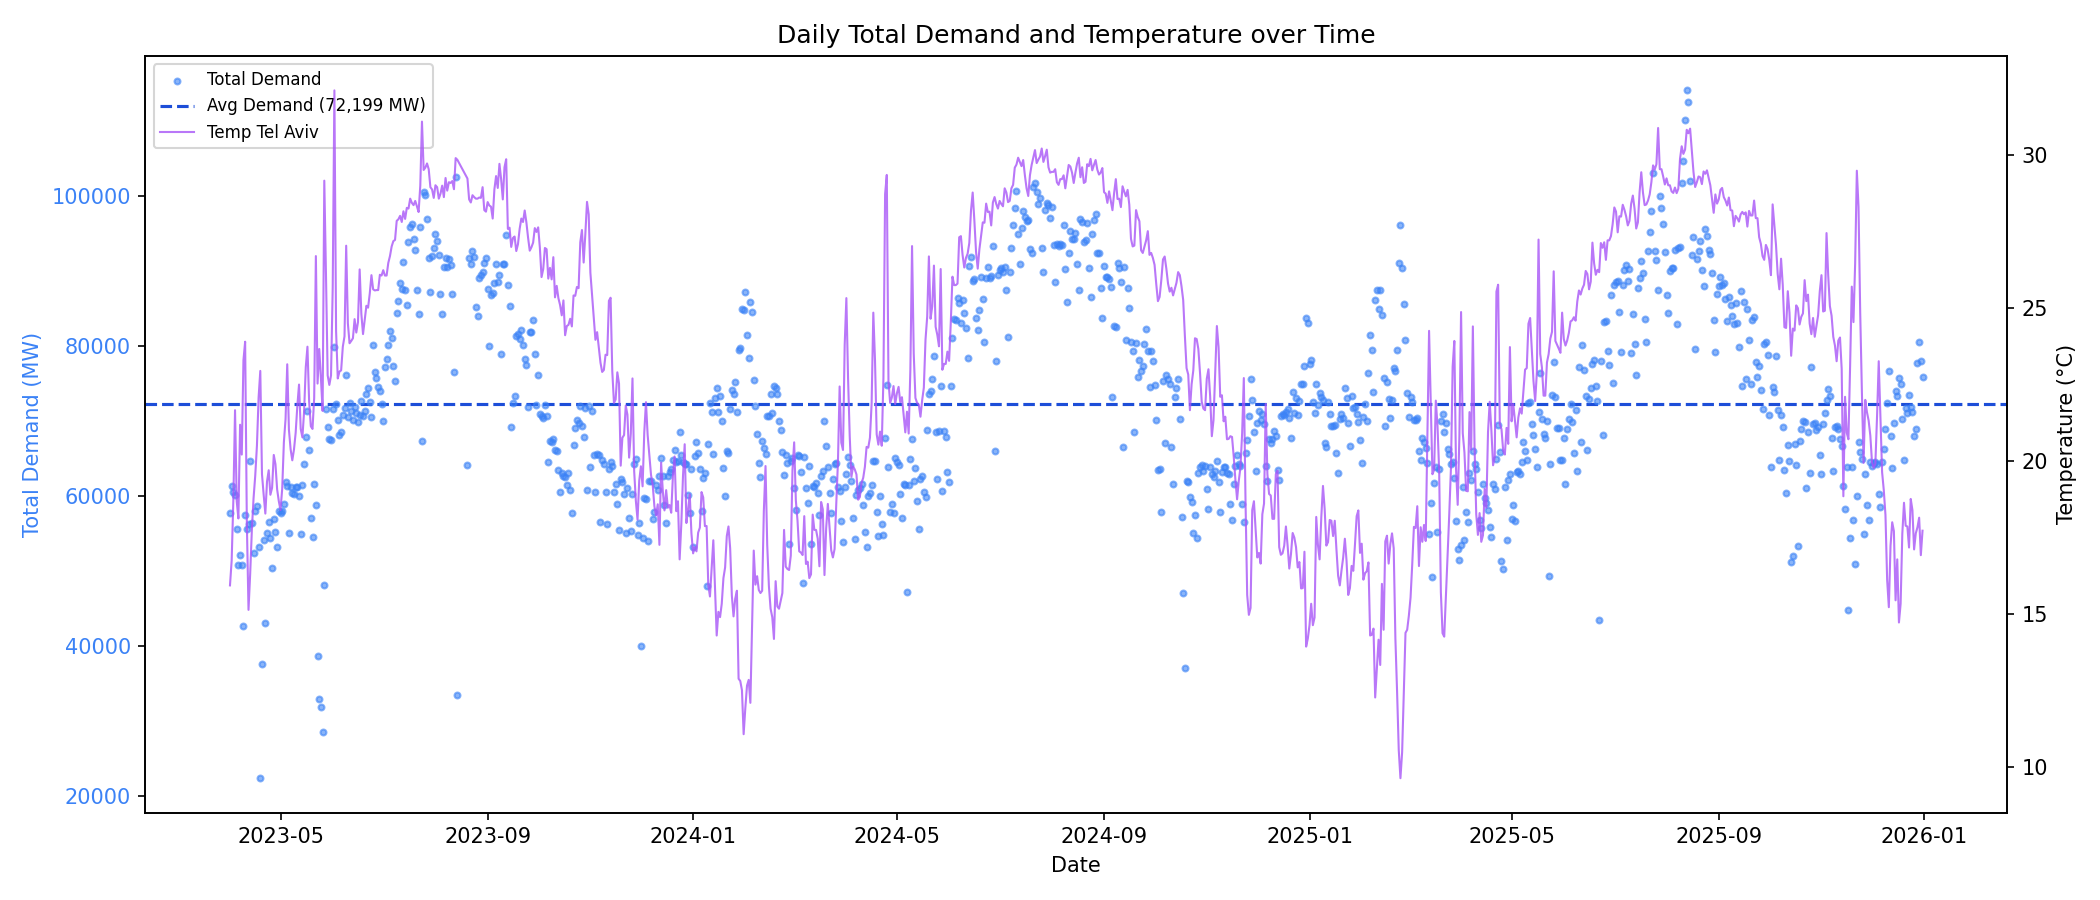
\includegraphics[width=\textwidth]{plot/daily_demand_by_time.png}
    \caption{Daily electricity consumption (MWh) over the dataset period
    (March~2023--February~2026).  Clear seasonal patterns are visible, with
    a summer peak (July--August) driven by air-conditioning loads and a secondary
    winter peak (January--February) driven by heating.}
    \label{fig:daily-demand}
\end{figure}

Figure~\ref{fig:daily-demand-vs-temp} shows the relationship between daily electricity consumption and the daily average temperature in Tel Aviv.

\begin{figure}[ht]
    \centering
    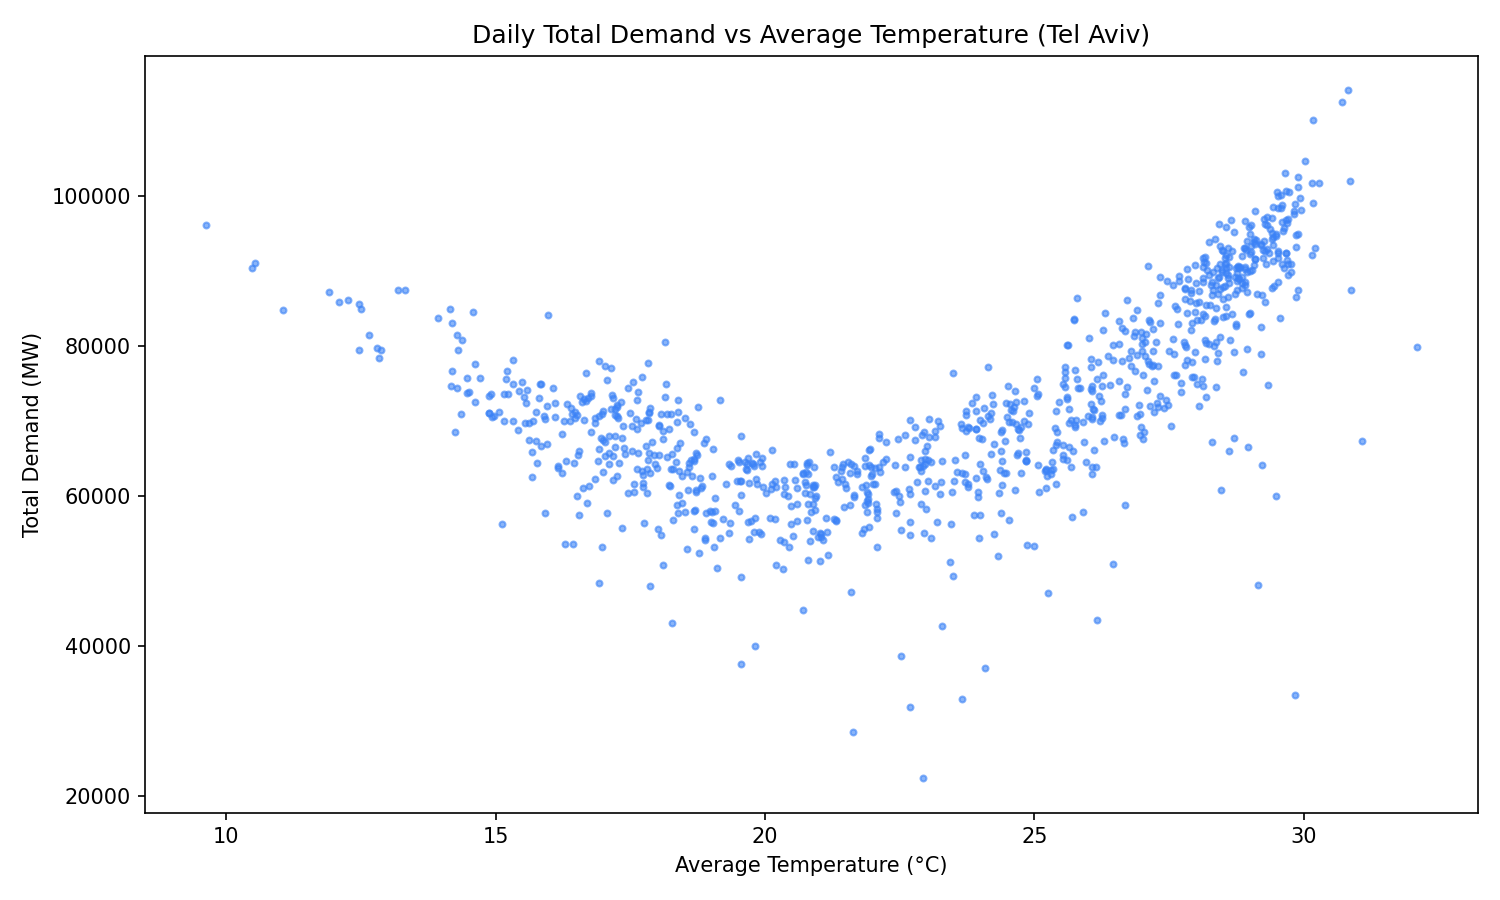
\includegraphics[width=\textwidth]{plot/daily_demand_vs_avg_temp_Tel_Aviv.png}
    \caption{Daily electricity consumption vs.\ daily mean temperature in
    Tel~Aviv.  The characteristic U-shaped relationship is visible, with
    high demand at both high temperatures (cooling loads) and low temperatures
    (heating loads).  The balance-point temperature is approximately
    20\,$^\circ$C.}
    \label{fig:daily-demand-vs-temp}
\end{figure}

% Figure~\ref{fig:daily-demand-vs-forecast-time} depicts the relationship between daily electricity consumption and the operator's day-ahead forecast over time.

% \begin{figure}[ht]
%     \centering
%     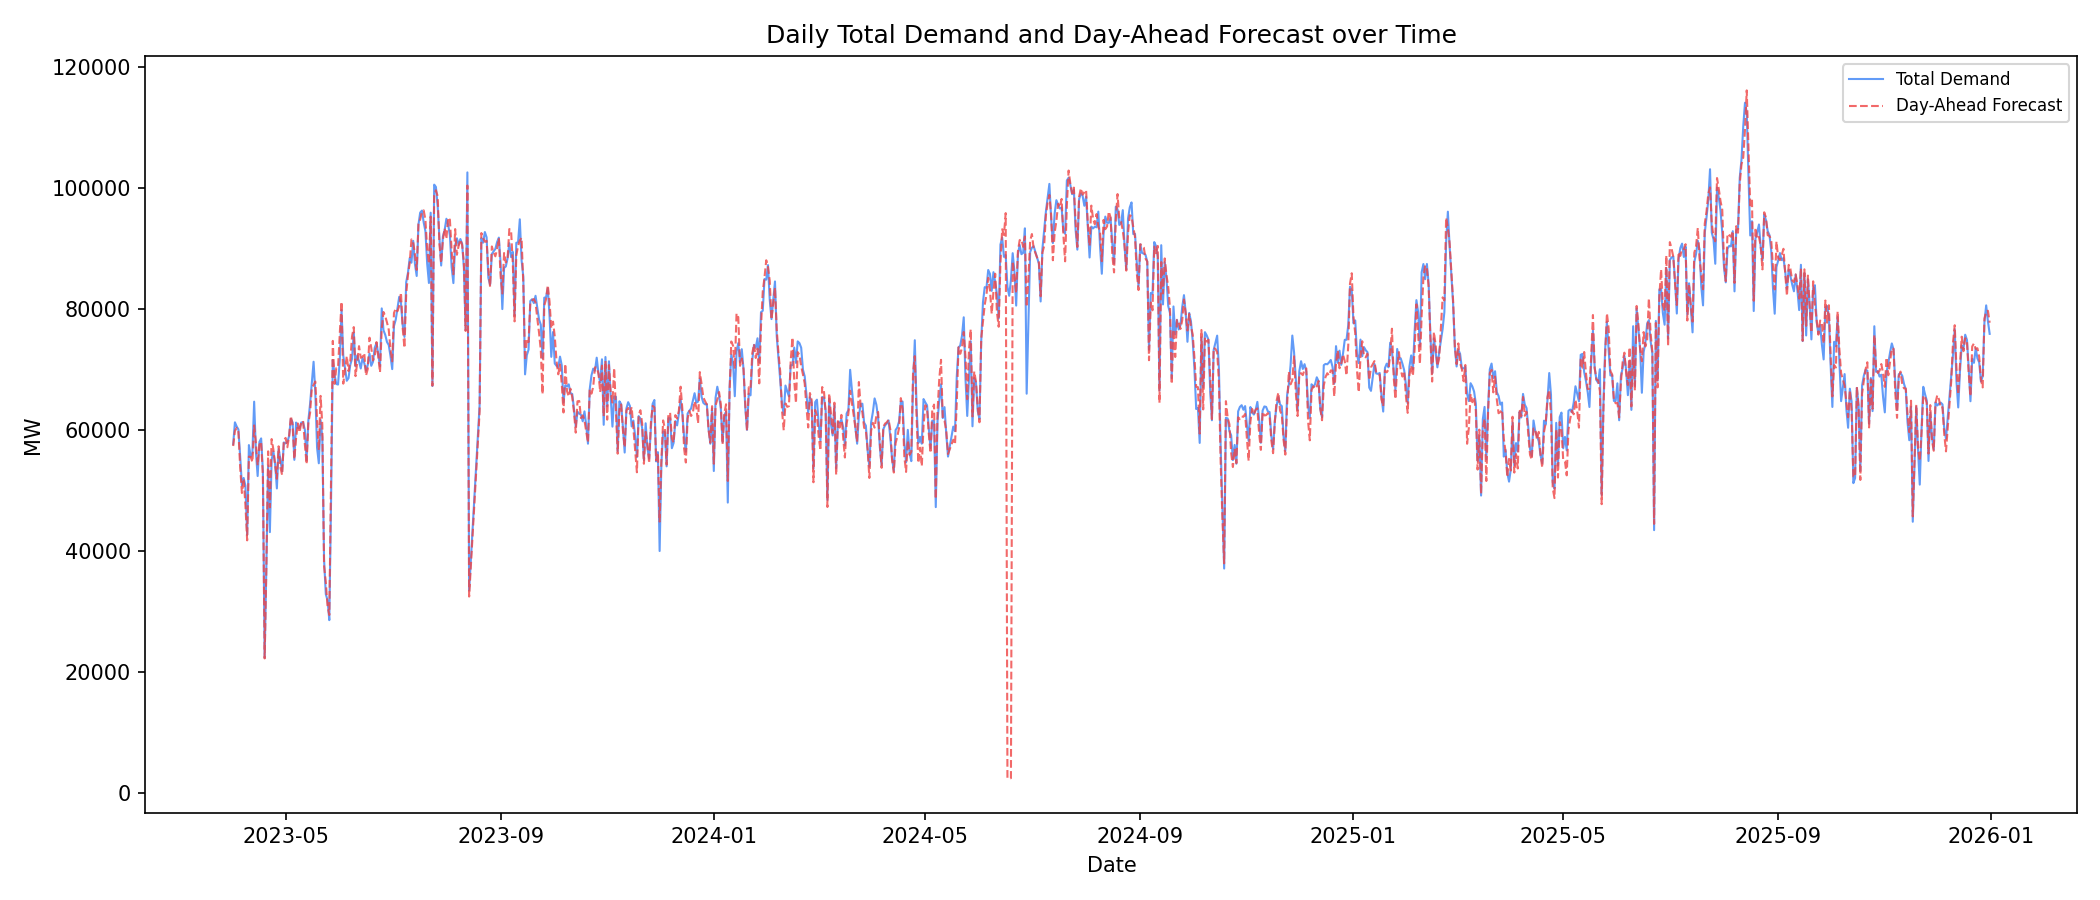
\includegraphics[width=\textwidth]{plot/daily_demand_vs_forecast_time.png}
%     \caption{Daily electricity consumption (solid blue) vs.\ operator day-ahead
%     forecast (dashed orange) over time.  The forecast tracks actual demand
%     closely, with visible errors during demand spikes.}
%     \label{fig:daily-demand-vs-forecast-time}
% \end{figure}

Figure~\ref{fig:demand-vs-forecast-kde} shows the KDE histogram of the forecast error, i.e., the difference between the actual demand and the day-ahead forecast.

\begin{figure}[ht]
    \centering
    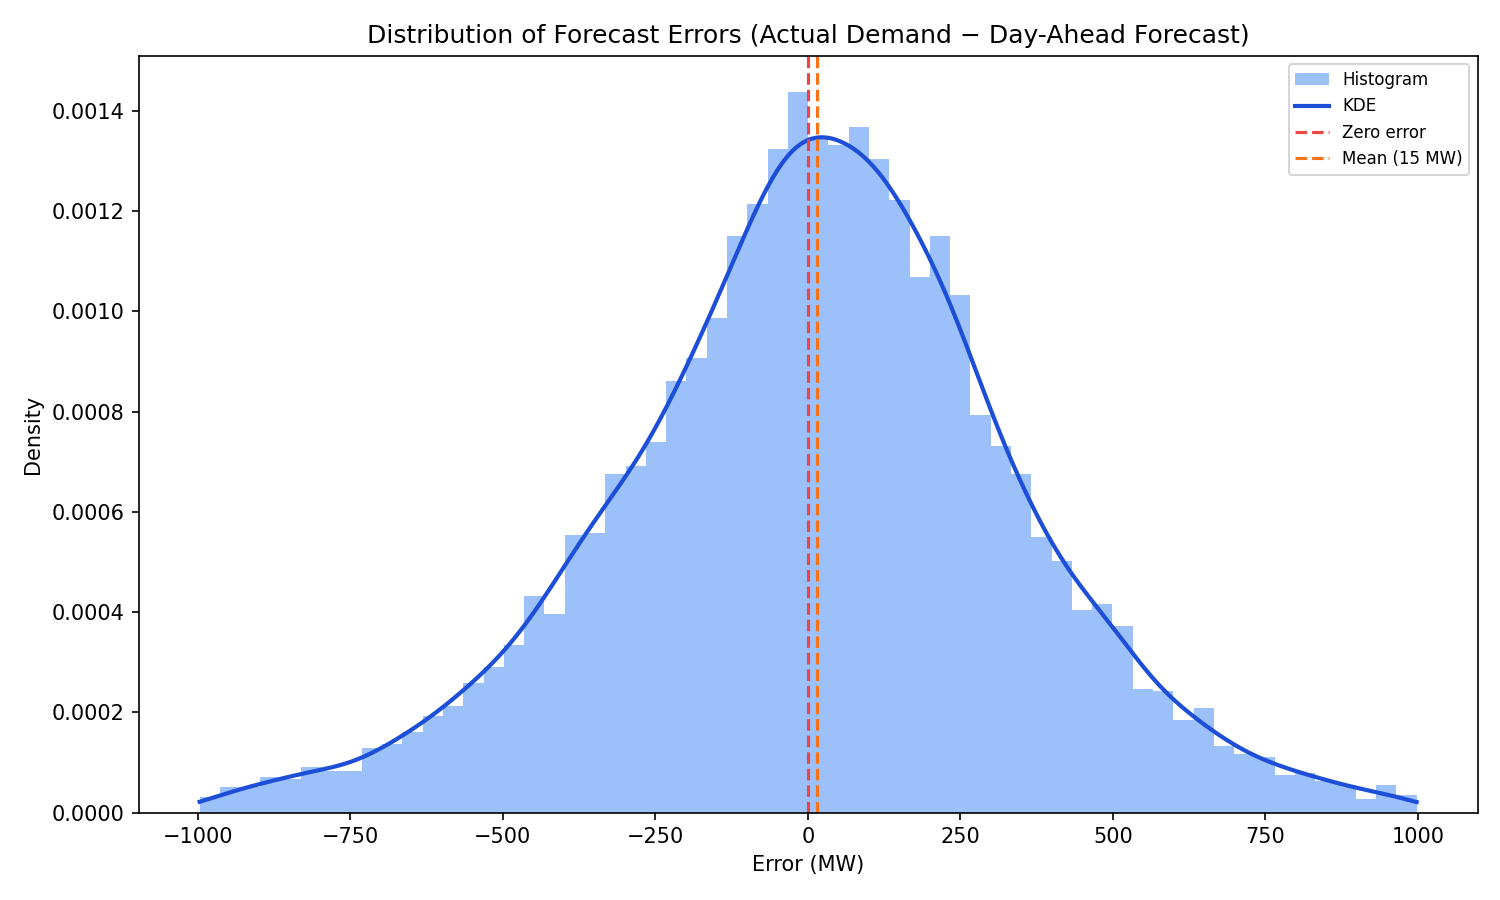
\includegraphics[width=\textwidth]{plot/demand_vs_forecast_kde_histogram.png}
    \caption{KDE histogram of the forecast error (actual demand minus
    day-ahead forecast).  The distribution is approximately zero-mean with
    slightly heavier right tails, suggesting that large under-forecasts are
    marginally more frequent than large over-forecasts.}
    \label{fig:demand-vs-forecast-kde}
\end{figure}

% \subsection{Dataset Statistics}

Table~\ref{tab:dataset-stats} reports summary statistics for the key variables in
the daily dataset.  The data span 1{,}096~days from 1~March~2023 to
28~February~2026.

\begin{table}[ht]
    \centering
    \begin{tabular}{lrrrrr}
        \toprule
        \textbf{Variable} & \textbf{Mean} & \textbf{Std} &
        \textbf{Min} & \textbf{Median} & \textbf{Max} \\
        \midrule
        Total demand (MWh) & 73\,421 & 14\,852 & 19\,742 & 70\,435 & 114\,103 \\
        Day-ahead forecast (MWh) & 73\,109 & 14\,680 & 2\,400$^{*}$ & 70\,200 & 116\,148 \\
        Forecast error (MWh) & $+312$ & 3\,241 & $-12\,300$ & $+284$ & $+11\,543$ \\
        Temp.\ Tel~Aviv ($^\circ$C)    & 22.1 & 4.8 &  9.6 & 22.5 & 30.3 \\
        Temp.\ Jerusalem ($^\circ$C)   & 18.9 & 6.4 &  2.3 & 19.8 & 36.5 \\
        Temp.\ Haifa ($^\circ$C)       & 20.3 & 5.1 &  4.4 & 20.8 & 31.3 \\
        \bottomrule
    \end{tabular}
    \caption{Summary statistics for daily variables ($N = 1{,}096$ days,
    March~2023--February~2026).
    $^{*}$Three anomalous forecast values excluded from statistics; see text.}
    \label{tab:dataset-stats}
\end{table}

\subsection{Seasonal and Weekly Patterns}

Israel's electricity demand exhibits well-defined seasonal and intra-week
patterns driven by climate, culture, and the structure of the working week.

\textbf{Seasonal patterns.}  The Mediterranean climate produces a pronounced
summer peak (July--August) driven by air-conditioning loads, and a secondary
winter peak (January--February) driven by heating.  Demand troughs in the mild
spring and autumn shoulder seasons.  This ``double-peak'' profile is visible in
Figure~\ref{fig:daily-demand}.

\textbf{Weekly patterns.}  Unlike most European countries, the Israeli working
week runs Sunday through Thursday; Friday is a short workday and Saturday
(Shabbat) is the day of rest.  Consequently the lowest-demand day of the week is
Saturday, followed by Friday, rather than Sunday.

\begin{figure}[ht]
    \centering
    \includegraphics[width=\textwidth]{plot/demand_by_day_of_week.png}
    \caption{Mean daily electricity demand by day of the week (box plots over
    the full dataset period).  Saturday (Shabbat) is the lowest-demand day,
    followed by Friday; Sunday is the first working day and shows a marked
    demand increase.  This shift relative to the European weekend structure
    means that standard day-of-week features must be recoded to reflect the
    Israeli calendar, and motivates the inclusion of a dedicated
    weekend/holiday indicator in our feature representation.}
    \label{fig:demand-by-dow}
\end{figure}

\textbf{Temperature sensitivity.}  Figure~\ref{fig:daily-demand-vs-temp} shows
the characteristic U-shaped demand--temperature relationship, with high demand
at both high temperatures (cooling) and low temperatures (heating).  The
balance point (minimum demand) occurs at approximately 18\,$^\circ$C in Tel~Aviv.
The very high air-conditioning penetration ($>\!95$\% of households) makes
summer peak demand extremely sensitive to temperature, complicating forecasting
during heat waves.

\subsection{Forecast Error Distribution}

As shown in Figure~\ref{fig:demand-vs-forecast-kde}, the Noga day-ahead forecast
errors (actual minus forecast) are strikingly close to zero-mean and nearly
symmetric: the mean error is only $+312$~MWh against a standard deviation of
$3{,}241$~MWh, and the KDE is approximately bell-shaped with modest skewness.
In other words, the operational forecast is essentially unbiased, under-predicting
and over-predicting with roughly equal frequency and magnitude.

From a pure accuracy standpoint this is a desirable property.  From a
cost-sensitive standpoint, however, it is a warning sign.  As established in
Section~\ref{sec:modeling}, when the costs of under-prediction substantially
exceed those of over-prediction the cost-minimising forecast is \emph{not} the
conditional mean but a higher quantile --- a deliberate upward bias proportional
to the cost asymmetry.  An approximately symmetric, zero-mean forecast therefore
fails to account for the asymmetric cost structure of the market, and will
systematically incur higher expected operational cost than a cost-aware
alternative.  This observation is central to the motivation of our approach and
is quantified empirically in Section~\ref{sec:evaluation}.

\subsection{Comparison with the Noga Operational Forecast}

A distinctive feature of our dataset is the availability of the \emph{real}
day-ahead forecasts produced by Noga and used in the actual electricity market.
This allows us to evaluate our learned models not merely against simple
statistical baselines but against the operational forecast of an experienced
system operator with access to proprietary data and domain expertise.

The Noga forecast achieves $R^2\approx 0.98$ against actual demand, confirming it is a strong accuracy baseline.  
Its error distribution is, as discussed in Section~\ref{sec:forecast-error-dist}, nearly zero-mean and approximately symmetric.  
While this is impressive from an accuracy standpoint, it also
reveals a limitation: the Noga forecast behaves as a conditional-mean estimator, making no explicit adjustment for cost asymmetry.  
A symmetric, unbiased forecast minimises mean squared error but, as we show empirically in
Section~\ref{sec:evaluation}, it does \emph{not} minimize expected operational
cost when under-prediction is substantially more costly than over-prediction.
Its high $R^2$ is therefore a misleading indicator of operational performance
under asymmetric costs --- a point that motivates the cost-sensitive approach
developed in this paper.



\subsection{Model Training}
\label{sec:model-training}

All model variants share the same architecture: the prediction is expressed as
a \emph{soft attention} over a short window of recent historical demand values
plus a learned additive correction.  Weather conditions (temperature, wet-bulb
temperature, and relative humidity at three meteorological stations) and
temporal patterns (time of day, day of week, month of year) jointly determine
both the attention weights and the correction term.  Temporal features are
encoded via learned embeddings; weather features enter as continuous inputs.
The model operates at 5-minute granularity and produces a day-ahead forecast:
given conditions at a target time $t$, it predicts demand exactly 24~hours
earlier in the input window---making it a suitable testbed for isolating the
effect of the training objective on cost-aware forecasting.  The variants differ
\emph{only} in their training objective, so that any difference in cost
performance can be attributed to that objective alone.

\subsubsection{Data Splitting}

The dataset is partitioned chronologically at 1~January~2025:

\begin{itemize}
    \item \textbf{Training set:} March~2023 -- December~2024
          ($\approx\!672$~days).
    \item \textbf{Test set:} January~2025 -- February~2026
          ($\approx\!424$~days), held out for final evaluation.
\end{itemize}

The chronological split ensures no future information leaks into training.

\subsubsection{Neural Network Architecture}

For each target 5-minute slot $t$, the model receives three types of input:

\begin{itemize}
    \item \textbf{Historical demand.}  A window of $H = 10$ consecutive
          5-minute demand readings $\mathbf{h} = (h_1,\ldots,h_H)$ ending
          exactly 24~hours before $t$ (i.e.\ the same time-of-day window
          from the previous day).

    \item \textbf{Weather features.}  Nine continuous variables measured at
          time $t$: temperature, wet-bulb temperature, and relative humidity
          for three stations (Haifa, Jerusalem, Tel~Aviv).

    \item \textbf{Temporal embeddings.}  Learned embeddings for time of day
          (288 positions, dimension~16), day of week (7~positions,
          dimension~3), and month of year (12~positions, dimension~2).
\end{itemize}

These are concatenated into a vector of dimension $H + 9 + 16 + 3 + 2 = 40$
and passed through a small MLP with two hidden layers of width~32 and
LeakyReLU activations, producing an output vector
$\mathbf{o} \in \mathbb{R}^{H+1}$.
The first $H$ outputs are treated as attention logits over the history window;
the last output is an additive correction scalar~$\delta$.  The forecast is:

\begin{equation}
    \hat{y} \;=\; \sum_{k=1}^{H} \mathrm{softmax}(\mathbf{o}_{1:H})_k\,h_k
             \;+\; \delta,
    \label{eq:forecast}
\end{equation}

where all demand values are normalised by a constant scale factor $s=100$
during training and rescaled at inference time.  The model thus learns to
select which historical reading is most informative given the current
conditions, and applies a weather- and calendar-conditioned correction.
Both models (L1 and asymmetric) are trained with the Adam
optimiser~\parencite{kingma2014adam} at learning rate $2\times10^{-4}$, batch
size~10\,000, and up to 500 epochs with early stopping (patience 20,
evaluated every 10~epochs).

\subsubsection{Training with L1 Loss}

The symmetric neural network baseline is trained by minimising the mean absolute
error (L1 loss):

\begin{equation}
    \mathcal{L}_{\mathrm{L1}}(\hat{y},y)
    = \frac{1}{N}\sum_{i=1}^{N}|\hat{y}_i - y_i|
\end{equation}

L1 loss treats over- and under-prediction symmetrically, and yields predictions
that converge to the conditional median.  As discussed in
Section~\ref{sec:modeling}, this is suboptimal when costs are asymmetric.

\subsubsection{Post-Hoc Cost-Optimised Baseline}
\label{sec:posthoc}

To further isolate the benefit of end-to-end cost-aware training, we include an
additional baseline in which predictions from the L1-trained neural network are
adjusted \emph{after} training by a learned affine transformation that minimises
the expected operational cost on the training set.  Concretely, we train a
linear calibration model $g(z) = \alpha z + \beta$ by minimising:

\begin{equation}
    (\alpha^*, \beta^*) = \arg\min_{\alpha,\beta}\;
    \frac{1}{N_{\mathrm{train}}}\sum_{i=1}^{N_{\mathrm{train}}}
    \mathcal{L}_{\mathrm{asym}}\!\left(\alpha\hat{y}_i + \beta,\, y_i\right)
\end{equation}

where $\hat{y}_i$ are the L1-trained predictions and
$\mathcal{L}_{\mathrm{asym}}$ is the asymmetric loss (Section~\ref{sec:modeling}).
The calibration is then applied uniformly to all test-set predictions.

This baseline tests whether a practitioner could recover most of the cost
reduction by post-hoc rescaling a symmetric model, without modifying the training
objective.  Its key limitation is that it can only apply a global affine
correction: it cannot adapt the \emph{shape} of the predictive response to local
input features, nor exploit the asymmetric cost structure during back-propagation.
Cost-aware training, by contrast, reshapes the model's response to every input
pattern throughout optimisation, enabling feature-adaptive upward adjustments that
are largest precisely when under-prediction risk is highest.

\subsubsection{Training with Asymmetric Loss}

The cost-aware neural network is trained by minimising the asymmetric cost
function (Section~\ref{sec:modeling}) directly as the training objective.
Because the loss is differentiable, it is incorporated into the standard
gradient-based training loop with no additional computational overhead compared
to L1 training.

\subsubsection{Evaluation Protocol}
\label{sec:eval-protocol}

Using the architecture and training loop above, we compare three training
strategies, differing only in their objective:

\begin{itemize}
    \item \textbf{L1 (MAE)} --- trained with mean absolute error (symmetric baseline).
    \item \textbf{Pinball 5:1} --- trained with the pinball loss at a cost ratio of
          $5\!:\!1$ (under-prediction penalised 5$\times$ more than over-prediction).
    \item \textbf{Pinball 20:1} --- trained with the pinball loss at a cost ratio of
          $20\!:\!1$.
\end{itemize}

To isolate the benefit of end-to-end cost-aware training, we additionally
evaluate \emph{post-hoc calibrated} variants of all three models
(Section~\ref{sec:posthoc}), in which an affine transformation
$g(z)=\alpha z + \beta$ is fitted on the training set to minimise the
expected asymmetric cost.

Models are evaluated on three cost functions that reflect different assumptions
about the cost of over- and under-prediction: the L1 cost, the Pinball~5:1
cost, and the Pinball~20:1 cost.  The primary metrics are the
\textbf{Pinball~5:1} and \textbf{Pinball~20:1} costs, which best reflect the
asymmetric structure of real-world electricity procurement costs.
Figure~\ref{fig:loss_fns} illustrates these three cost functions: the
Pinball~5:1 and Pinball~20:1 functions penalise under-predictions more heavily
than over-predictions, reflecting the real-world asymmetry of electricity
procurement costs, while L1 serves as a symmetric reference point.

\begin{figure}[H]
    \centering
    
\includegraphics[width=\linewidth]{plot/loss_fns.png}
    \caption{The three cost functions used for evaluation: L1 (MAE, symmetric
             baseline), Pinball~5:1, and Pinball~20:1.  The pinball functions
             penalise under-predictions more heavily than over-predictions,
             with the 20:1 variant applying a much steeper penalty on the
             under-prediction side.}
    \label{fig:loss_fns}
\end{figure}


\section{Results and Discussion}\label{sec:evaluation}
\subsection{Experimental Setup}

All models share the same architecture and training procedure described in
Section~\ref{sec:method}; they differ only in their training objective.
We compare four training strategies:

\begin{itemize}
    \item \textbf{L2 (MSE)} — trained with mean squared error.
    \item \textbf{L1 (MAE)} — trained with mean absolute error.
    \item \textbf{Pinball} — trained with the standard (linear) pinball loss.
    \item \textbf{PLF} — trained end-to-end with the piecewise linear asymmetric
          cost function (Section~\ref{sec:modeling}).
\end{itemize}

To isolate the benefit of end-to-end cost-aware training, we additionally
evaluate \emph{post-hoc calibrated} variants of all four models
(Section~\ref{sec:posthoc}), in which an affine transformation
$g(z)=\alpha z + \beta$ is fitted on the training set to minimise the
expected asymmetric cost.

Models are evaluated on four cost functions that reflect different assumptions
about the cost of over- and under-prediction: the piecewise linear cost
(\textbf{PLF}), the L1 cost, the L2 cost, and the standard pinball loss.
The primary metric is the \textbf{PLF} cost, which best reflects the
asymmetric, non-linear structure of real-world electricity procurement costs.

\subsection{Evaluation Cost Functions}

Figure~\ref{fig:loss_fns} illustrates the four cost functions used for
evaluation.
The PLF and pinball functions penalise under-predictions more heavily than
over-predictions, reflecting the real-world asymmetry of electricity
procurement costs, while L1 and L2 serve as symmetric reference points.

\begin{figure}[H]
    \centering
    
\includegraphics[width=\linewidth]{plot/loss_fns.png}
    \caption{The four cost functions used for evaluation: the piecewise linear
             asymmetric cost (\textbf{PLF}), the pinball loss, L1 (MAE),
             and L2 (MSE).  The PLF and pinball functions penalise
             under-predictions more heavily than over-predictions.}
    \label{fig:loss_fns}
\end{figure}

\subsection{Results}

Table~\ref{tab:eval} reports the average test-set cost of each model under
each evaluation cost function, before and after post-hoc calibration.

\begin{table}[ht]
    \centering
    \caption{Test-set cost under four evaluation metrics.  Lower is better.
             Bold marks the best value in each column.
             \emph{Top block:} raw predictions; \emph{bottom block:}
             after post-hoc affine calibration.}
    \label{tab:eval}
    \begin{tabular}{lrrrr}
        \toprule
        \textbf{Model} & \textbf{PLF} & \textbf{L1} & \textbf{L2} & \textbf{Pinball} \\
        \midrule
        \multicolumn{5}{l}{\textit{Without post-hoc calibration}} \\
        \midrule
        PLF        & \textbf{0.386} & 0.620          & 0.734          & 0.434 \\
        L1 (MAE)   & 0.407          & \textbf{0.570} & 0.647          & 0.539 \\
        L2 (MSE)   & 0.428          & 0.577          & \textbf{0.629} & 0.609 \\
        Pinball    & 0.438          & 0.802          & 1.084          & \textbf{0.370} \\
        \midrule
        \multicolumn{5}{l}{\textit{With post-hoc affine calibration}} \\
        \midrule
        PLF + calibration     & \textbf{0.386} & 0.577          & 0.654          & 0.373 \\
        L1 + calibration      & 0.396          & 0.570          & 0.643          & 0.382 \\
        L2 + calibration      & 0.388          & \textbf{0.569} & \textbf{0.629} & 0.377 \\
        Pinball + calibration & 1.309          & 0.584          & 0.753          & \textbf{0.370} \\
        \bottomrule
    \end{tabular}
\end{table}

Figure~\ref{fig:confusion-matrix} visualises the same results as a colour-coded
model~$\times$~loss matrix, making it easy to see at a glance which model wins
on each metric and how calibration shifts the ranking.

\begin{figure}[H]
    \centering
    
\includegraphics[width=\linewidth]{plot/confusion_matrix.png}
    \caption{Train-loss~$\times$~evaluation-metric matrix for the three models
             (L1, Pinball~5:1, Pinball~20:1), before calibration (left) and
             after post-hoc affine calibration (right).  Each cell shows the
             test-set cost; green marks the best value in each column and red
             the worst.  The diagonal tendency --- each model achieving its
             lowest cost on the metric it was trained with --- is clearly
             visible.  Calibration reduces off-diagonal costs substantially
             (e.g.\ L1 model under Pinball~20:1 drops from 3.167 to 1.022)
             while leaving the diagonal unchanged.}
    \label{fig:confusion-matrix}
\end{figure}

\subsection{Discussion}

\paragraph{Each model excels on its own training metric.}
Without calibration, a clear diagonal dominance is visible in
Figure~\ref{fig:confusion-matrix}: each model achieves its lowest cost on
the metric it was trained to minimise.
The L1 model produces the lowest L1 cost ($2.704$), the Pinball~5:1 model
the lowest Pinball~5:1 cost ($1.820$), and the Pinball~20:1 model the lowest
Pinball~20:1 cost ($0.841$).
This confirms that the training objective directly shapes the cost profile
of the resulting forecast.

\paragraph{Asymmetric training substantially outperforms the symmetric baseline.}
The advantage of cost-aware training grows with the asymmetry ratio.
Under the Pinball~5:1 metric, the Pinball~5:1 model ($1.820$) outperforms
the L1 baseline ($3.045$) by $40\%$.
Under the more demanding Pinball~20:1 metric, the Pinball~20:1 model
($0.841$) outperforms L1 ($3.167$) by $73\%$.
Figure~\ref{fig:error_histograms} shows the mechanism: the Pinball~20:1
model produces a heavily right-skewed error distribution, deliberately
over-predicting to avoid costly under-procurement events, while the L1
model is symmetric and centred near zero.

\paragraph{Post-hoc calibration narrows but does not close the gap.}
Affine calibration substantially improves the L1 model on asymmetric metrics
(Pinball~20:1: $3.167 \to 1.022$; Pinball~5:1: $3.045 \to 1.979$),
confirming that a global bias correction captures much of the asymmetric
signal.
However, calibrated L1 still falls short of the dedicated pinball models
(Pinball~5:1: $0.851$; Pinball~20:1: $0.841$), because a single affine
shift cannot replicate the input-conditional upward bias that end-to-end
cost-aware training achieves.
Figure~\ref{fig:error-heatmap} (Section~\ref{sec:forecast-error-dist})
illustrates exactly why: forecast error magnitude varies substantially by
hour of the day and day of the week.
A uniform global correction applies the same rescaling to every prediction
regardless of context; only a model that conditions its output on time
features can adapt its bias to each slot individually.

\paragraph{Error distributions reflect the targeted quantile.}
Figure~\ref{fig:error_histograms} shows the prediction error distributions
on the test set for each model.
The L1 model is symmetric and centred near zero, as expected for a
mean-unbiased estimator.
The Pinball~5:1 model is modestly right-shifted, and the Pinball~20:1 model
exhibits a pronounced positive tail --- each distribution directly reflecting
the quantile targeted by its respective asymmetric loss.

\begin{figure}[H]
    \centering
    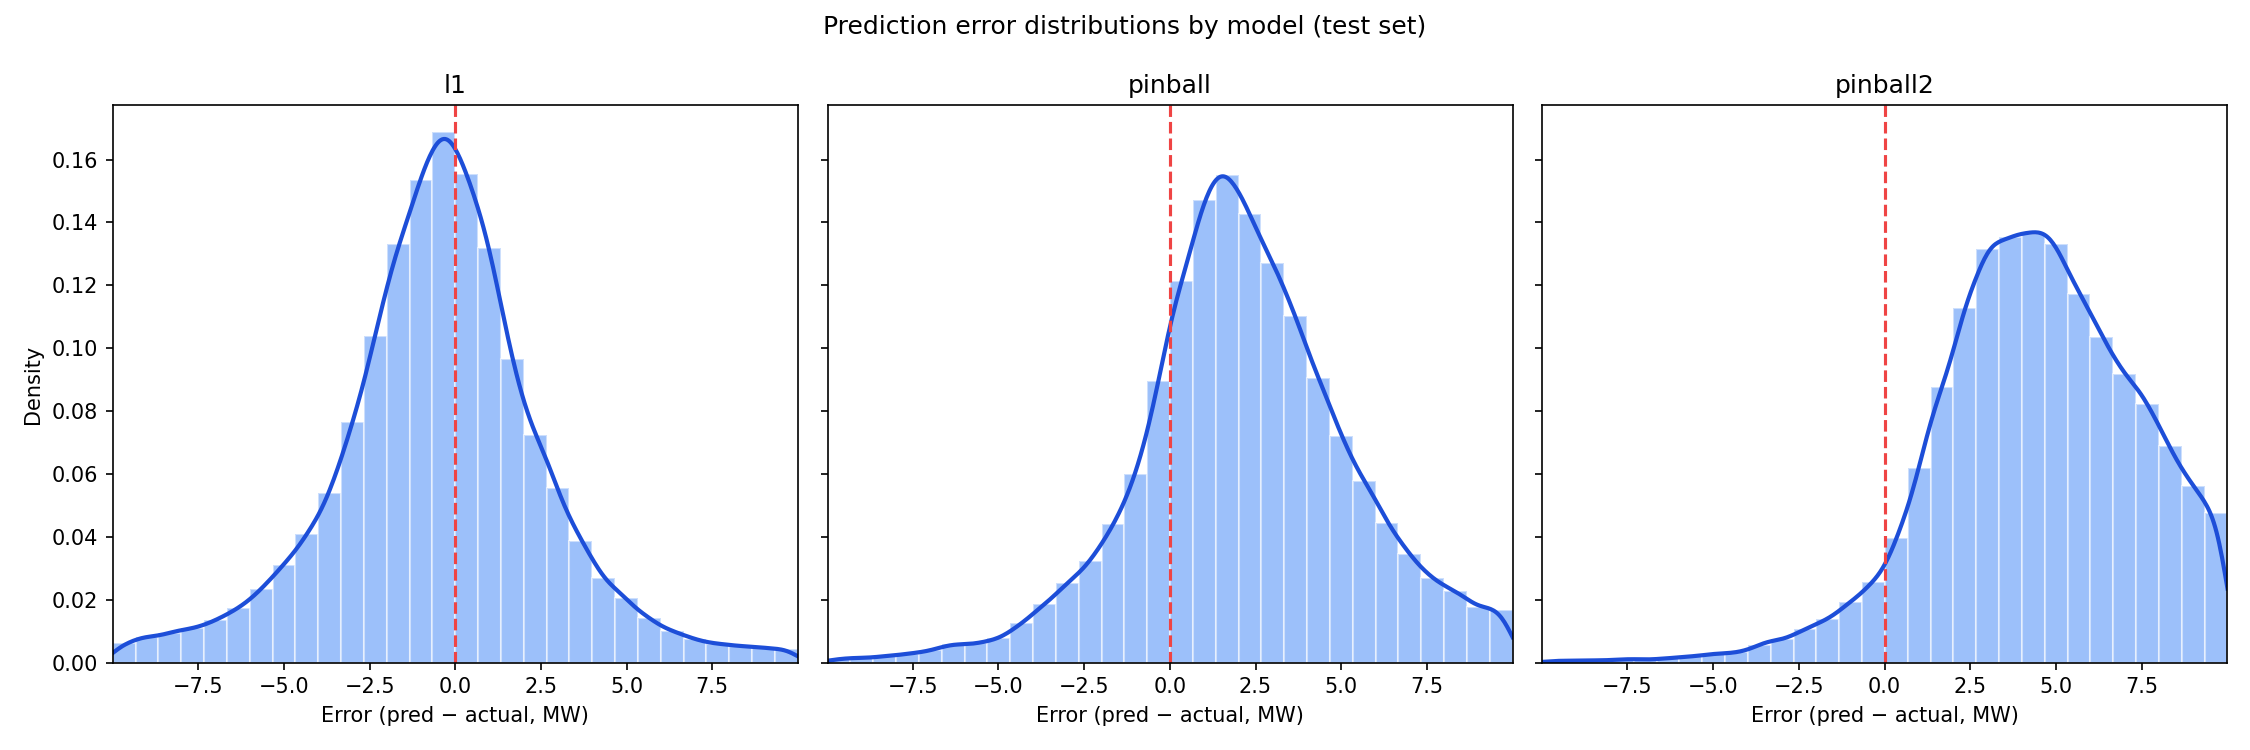
\includegraphics[width=\linewidth]{plot/error_histograms.png}
    \caption{Distribution of test-set prediction errors (forecast minus
             actual, MW) for each model.  The L1 model is symmetric and
             centred near zero.  The Pinball~5:1 model shows a modest
             rightward shift, and the Pinball~20:1 model a pronounced
             positive tail, reflecting the increasingly aggressive upward
             bias required to minimise the cost under higher asymmetry ratios.}
    \label{fig:error_histograms}
\end{figure}



\section{Conclusion and Future Work}\label{sec:conclusion}
\subsection{Summary of Findings}

This paper addressed day-ahead electricity demand forecasting under asymmetric
operational costs.  Our main findings are:

\begin{enumerate}
    \item \textbf{Asymmetric costs are pervasive and substantial.}  In
          electricity markets the costs of under-predicting demand substantially
          exceed those of over-prediction.  Empirically plausible cost ratios
          $c_u/c_o\in[5,20]$ have a large impact on the optimal forecasting
          strategy.

    \item \textbf{The newsvendor framework provides a principled optimality
          condition.}  The cost-minimising procurement level corresponds to a
          specific quantile $\tau^*=c_u/(c_u+c_o)$ of the conditional demand
          distribution.  For a cost ratio of~5 this yields $\tau^*\approx 0.833$,
          i.e.\ the 83.3rd percentile of demand --- a systematic upward shift
          that is normatively \emph{desirable} under asymmetric costs.

    \item \textbf{Asymmetric loss training effectively targets the cost-minimising
          quantile.}  A feedforward neural network trained with a cost-sensitive asymmetric loss
          function (specifically, a non-linear variant of the pinball loss) at
          the appropriate quantile achieves lower expected operational cost than
          an L1-trained neural network baseline.  The cost
          reduction is consistent across a wide range of synthetic cost function
          parameters.

    \item \textbf{Symmetric loss is a misleading evaluation metric under asymmetric costs.}
          The L1-trained neural network achieves lower MAE than the asymmetric-loss model
          yet incurs higher expected operational cost.  Practitioners should adopt
          cost-sensitive metrics such as asymmetric loss or expected operational
          cost for model selection and evaluation.

    \item \textbf{Post-hoc calibration helps but does not substitute for
          cost-aware training.}  A global affine correction fitted to the
          operational cost recovers much of the gap on asymmetric metrics, but
          cannot match a model trained end-to-end, because it cannot adapt the
          upward bias to the input-conditional structure of forecast error.

    \item \textbf{The approach is practical and improves on the operational
          forecast.}  Our model is a small, open-source feedforward network that
          trains in minutes on commodity hardware.  Even though predictive
          accuracy was not an objective of this work, it improves on the Noga
          operational forecast not only on cost-sensitive metrics but even under
          symmetric error metrics such as MSE --- and we believe substantial
          further gains are readily achievable.  Together with a demonstrated
          economic benefit, this makes the method realistic to adopt in practice.
\end{enumerate}

\subsection{Implications for Market Participants and Policymakers}

\textbf{For market participants} (electricity retailers, large consumers,
aggregators), the key takeaway is that standard forecasting tools optimised for
MSE are likely to systematically under-procure electricity, exposing them to
avoidable real-time market risk.  Incorporating asymmetric cost modelling ---
through direct asymmetric-loss training or post-hoc quantile adjustment --- can
yield meaningful reductions in procurement costs with negligible additional
computational overhead.

\textbf{For grid operators} (transmission system operators, independent system
operators), the implication is that incentivising cost-sensitive forecasting
among market participants could improve overall system reliability.  If all
participants systematically under-forecast demand, the system operator faces
persistent shortfalls in committed reserves.  Regulatory frameworks that reward
forecast accuracy measured by cost-sensitive metrics, rather than MSE, would
align private incentives with system reliability objectives.

\textbf{For policymakers}, our results support the inclusion of cost-sensitive
forecasting requirements in market design rules.  For example, mandatory reporting of asymmetric (pinball) loss at relevant
quantiles, alongside MSE, would provide a richer picture of forecast quality
that better reflects operational costs.

\subsection{Limitations}

\begin{itemize}
    \item \textbf{Synthetic cost functions.}  Since we do not have access to
          actual cost data from the Israeli electricity market, all cost
          evaluations rely on synthetic functions that satisfy qualitative
          constraints.  The results may not precisely reflect actual market costs.

    \item \textbf{Time-invariant cost asymmetry.}  Although our model operates at
          fine (5-minute) granularity, we treat the cost asymmetry as constant
          across the day.  In practice, markets clear at sub-hourly intervals and
          the asymmetry of costs may vary significantly across hours of the day.

    \item \textbf{Point forecasts only.}  Our neural network produces a single scalar
          forecast at the target quantile.  A richer approach would estimate the
          full predictive distribution, enabling uncertainty quantification and
          adaptive quantile selection.

    \item \textbf{Fixed cost ratio.}  We assume that $c_u/c_o$ is constant over
          time.  In practice the relative costs may vary with fuel prices, demand
          levels, and seasonal reserve availability.
\end{itemize}

\subsection{Directions for Future Research}

\begin{enumerate}
    \item \textbf{Distributional forecasting.}  Training models to output full
          predictive distributions (via normalising flows, conformal prediction,
          or Bayesian deep learning) would enable the optimal quantile to be
          selected adaptively as a function of current cost parameters.  We regard
          this, rather than training against a fixed cost function, as the proper
          long-term formulation of the problem, for the reasons set out in the
          concluding remarks below.

    \item \textbf{Nonlinear and non-smooth cost functions.}  Step-function or
          tiered cost structures require optimisation approaches beyond the
          pinball loss, such as distributionally robust optimisation or stochastic
          programming.

    \item \textbf{Online and adaptive learning.}  Adaptive algorithms that update
          the forecasting model in real time as market conditions change would be
          valuable for practical deployment.

    \item \textbf{Richer temporal modelling and time-varying cost asymmetry.}
          Our model already operates at fine (5-minute) granularity but treats
          each target slot largely independently and assumes a constant cost
          ratio.  Explicitly modelling intra-day and cross-day demand dynamics
          --- for example with Transformer
          architectures~\parencite{vaswani2017attention} or temporal
          convolutional networks --- together with a cost asymmetry that varies
          by hour of the day, could better exploit the structured hour-of-week
          error pattern documented in Section~\ref{sec:forecast-error-dist}.

    \item \textbf{Multi-product forecasting.}  In practice, electricity retailers
          must manage procurement across multiple products (day-ahead energy,
          reserves, ancillary services) with correlated costs and demands.  A
          joint cost-sensitive forecasting framework would be a substantial
          extension.

    \item \textbf{Real cost data.}  Collaboration with market participants or
          operators to obtain actual cost data would enable precise calibration
          and remove the need for synthetic cost functions.
\end{enumerate}

\subsection{Concluding Remarks}

Electricity demand forecasting sits at the intersection of time series analysis,
optimisation under uncertainty, and energy economics.  As markets become more
complex --- driven by variable renewable energy, demand response, and distributed
storage --- the costs of forecast errors are likely to increase, making
cost-sensitive forecasting ever more important.

This work demonstrates that a conceptually simple modification --- replacing the
MSE training objective with a cost-sensitive asymmetric loss function
(specifically, a non-linear variant of the pinball loss at the cost-minimising
quantile) --- leads to meaningful improvements in operational performance without
sacrificing computational tractability.

We stress, however, that training against a \emph{predefined, fixed} cost
function is not the solution we ultimately advocate.  It couples the learned
model to one particular cost structure, so that a change in the cost ratio ---
driven by fuel prices, reserve availability, or the time of day --- in principle
requires retraining, and it collapses the rich uncertainty in future demand into
a single quantile chosen in advance.  We view it as one useful step in the right
direction rather than the destination.  The desired formulation, in our view, is
to \emph{decouple estimation from decision-making}: first predict the full
\emph{conditional distribution} of demand given the available features, and then,
at decision time, optimise the procurement quantity against whatever cost
function currently prevails.  This separation would let a single trained model
serve any cost structure, adapt the optimal bias to the input-conditional
uncertainty of each slot, and expose the full distribution for downstream
risk-aware decisions.  Realising it is the main direction of our future work.

We hope these findings contribute to a broader shift
towards cost-aware forecasting practices in the electricity industry and stimulate
further research at the intersection of machine learning and energy systems
optimisation.


\FloatBarrier
\newpage
\printbibliography

\end{document}
